\documentclass{article}

% Packages
\usepackage{fullpage}
\usepackage{amssymb}
\usepackage{multicol}
\usepackage{amsmath}
\usepackage{amsfonts}
\usepackage{bm}
\usepackage{float}
\usepackage{tikz}
\usepackage{xcolor}
\usetikzlibrary{shapes.geometric, positioning, arrows, intersections}
\usepackage{amsthm}
\usepackage{tcolorbox}
\usepackage{hyperref}
\hypersetup{
    colorlinks=true, %set true if you want colored links
    linktoc=all,     %set to all if you want both sections and subsections linked
    linkcolor=black,  %choose some color if you want links to stand out
}
\usepackage{esint}
\usepackage{tikz-3dplot}
\usepackage{pgfplots}
\usetikzlibrary{decorations.markings,arrows}
\pgfplotsset{compat=newest}


\definecolor{darkolivegreen}{rgb}{0.33, 0.42, 0.18}

% Macros
\newcommand{\R}{\mathbb{R}}
\newcommand{\N}{\mathbb{N}}
\newcommand{\Q}{\mathbb{Q}}
\newcommand{\sub}{\subset}
\renewcommand{\vec}[1]{\underline{\textbf{#1}}}
\newcommand{\uvec}[1]{\hat{\underline{\textbf{#1}}}}
\newcommand{\veci}{\bm{\hat{\imath}}}
\newcommand{\vecj}{\bm{\hat{\jmath}}}
\newcommand{\veck}{\bm{\hat{k}}}
\newcommand{\vecn}{\underline{\mathbf{\hat{n}}}}
\newcommand{\e}{\varepsilon}
\renewcommand{\th}{\vartheta}
\newcommand{\de}{\delta}
\renewcommand{\k}{\kappa}
\newcommand{\p}{\Phi}
\newcommand{\pa}{\partial}
\newcommand{\kd}{\delta_{i, j}}
\newcommand{\at}{\e_{i, j, k}}
\newcommand{\nab}{\underline{\nabla}}
\newcommand{\grad}{{\nab}\, f}
\newcommand{\pd}[2]{\frac{\partial #1}{\partial #2}}
\newcommand{\fd}[2]{\frac{d #1}{d #2}}
\renewcommand{\div}{\nab \cdot}
\newcommand{\curl}{\nab \times}

%ToC stuff
\newtheorem{example}{Example}
\newtheorem{solution}{Solution}
%\newtheorem{definition}{Definition}[subsection]
\newtheorem{corollary}{Corollary}

\tcbuselibrary{theorems}
\newtcbtheorem[number within=section]{theorem}{Theorem}%
{colback=green!5,colframe=green!35!black,fonttitle=\bfseries}{th}
\newtcbtheorem[number within=section]{definition}{Definition}%
{colback=blue!5,colframe=blue!35!black,fonttitle=\bfseries}{def}

\title{Vector Calculus Week 3 - Differentiating}
\author{James Arthur}

\begin{document}
\maketitle
\tableofcontents\newpage

\multicols{2}

\section{Differentiating Scalar Fields}

\noindent\begin{definition}{Partial Differentiation}{}
  Let $\displaystyle{U\sub \R^n}$ be an open set. The $\displaystyle{\pd{f}{x_1}, \dots, \pd{^n f}{x_n}}$ partial derivatives of $f(x_1, \dots, x_n)$ which at point $\underline{x}$ are defined by:
  $$ \pd{f}{x_j} =$$ $$ \lim_{h\to 0}{\frac{f(x_1, \dots, x_j + h, \dots, x_n) - f(x_1,\dots,x_n)}{h}}$$
  where the limit exists for $j$ from $1$ to $n$.
\end{definition}\vspace{10pt}

\begin{example}{
  If $f(x, y) = x^2y + y^3$, then find $\displaystyle{\pd{f}{x}}$ and $\displaystyle{\pd{f}{y}}$
}\end{example}\begin{solution}{
  We can simply work out that:
  $$ \pd{f}{x} = 2xy $$
  $$ \pd{f}{y} = x^2 + 3y^2 $$
}\end{solution}\vspace{10pt}

To say that a partial derivative shall be evaluated at a point $(x_0, y_0)$, we write; $\displaystyle{\pd{f}{x}\Bigr|_{(x_0,y_0)}}$

\subsection{Equations of Tangent planes}
\noindent\begin{definition}{Tangent Plane}{}
Let $f : \R^2 \to \R$ be differeniable at $(x_0, y_0)$, the plane described by:
$$ z_p = f(x_0,y_0) + \pd{f}{x_0}\Bigr|(x - x_0) + \pd{f}{y}\Bigr|(y - y_0) $$
is called the tangent plane of $f$ at $(x_0, y_0)$.
\end{definition}\vspace{10pt}

\begin{figure}[H]
  \centering
  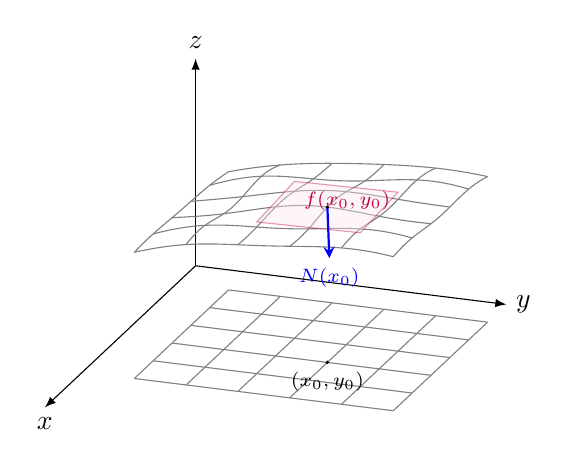
\begin{tikzpicture}[font=\sffamily,declare function={%
      f(\x,\y)=3+.075*cos(\x*100)*cos(\y*100)-.035*(\y-5)^2-.01*(\x-5)^2;
      g(\x) = .075*(\x-4)^2+4;
      h(\x) = .02*(\x-4)^3-.2*(\x-4)+4;
      t(\x,\y)=f(4,4) -0.05*(\x-4) + 0.02*(\y-4); }, scale=0.7]

      \tdplotsetmaincoords{70}{110}

      \begin{scope}[tdplot_main_coords]
          \draw[-latex] (0,0,0) -- (8,0,0) node[anchor=north] {$x$};
          \draw[-latex] (0,0,0) -- (0,6,0) node[anchor=west] {$y$};
          \draw[-latex] (0,0,0) -- (0,0,4) node[anchor=south] {$z$};

          %Grid
          \foreach \X in {1,...,6}
          {
              \draw[thin,gray] plot[variable=\x,samples=60,smooth,domain=1:6] ({\X},{\x},0);
              \draw[thin,gray] plot[variable=\x,samples=60,smooth,domain=1:6] ({\x},{\X},0);
              \draw[thin,gray] plot[variable=\x,samples=60,smooth,domain=1:6] ({\X},{\x},{f(\X,\x)});
              \draw[thin,gray] plot[variable=\x,samples=60,smooth,domain=1:6] ({\x},{\X},{f(\x,\X)});
          }
          % Tangent plane
          \fill[purple!10,opacity=0.4,draw=purple] (3,3,{t(3,3)}) -- (3,5,{t(3,5)}) -- (5,5,{t(5,5)}) -- (5,3,{t(5,3)}) -- (3,3,{t(3,3)}) node[anchor=north west,purple,opacity=1] {\scriptsize $f(x_0, y_0)$};

          % Vector fields
          \draw[->,>=stealth,thick,blue] (4,4,{f(4,4)}) -- (3.95,4.02,2) node [below] {\scriptsize $N(x_0)$};

          % Points
          \fill[black] (4,4,0) circle (1pt) node[anchor=north] {\scriptsize $(x_0, y_0)$};
          \fill[black] (4,4,{f(4,4)}) circle (1pt) node[anchor=north east] {};
      \end{scope}
  \end{tikzpicture}
\end{figure}

\noindent\begin{definition}{}{}
  Let $f$ be a function $f: \R^2 \to \R$ we say that $f$ is differentiable at $(x_0, y_0)$, if $\pd{f}{x}$ and $\pd{f}{y}$ exists at $(x_0, y_0)$ and if
  $$ \lim_{(x, y) \to (x_0, y_0)}{\frac{f(x, y) - z_p}{\| (x, y) - (x_0, y_0) \|}} $$
  then $z_p$ is a good approximation of $f$.
\end{definition}\vspace{10pt}

\subsection{Gradient of a scalar field}
\noindent\begin{definition}{}{}
  The gradient of a scalar field is a vector field with a direction that is perpendicular to the level surface and pointing in the direction of increasing $f$, with a magnitude equal to the rate of change of $f$ in this direction.
  $$ \grad = \pd{f}{x}\veci + \pd{f}{y}\vecj + \pd{f}{z}\veck $$
\end{definition}\vspace{10pt}

Consider an infitesimal change in the position in space from $\vec r$ to $d\vec r$. This results in a small change in the value of $f$, from $f$ to $f+df$.
\begin{align*}
  df &= \pd{f}{x}dx + \pd{f}{y}dy + \pd{f}{z}dz\\
  &= \grad \cdot d\vec r
\end{align*}

\begin{figure}[H]
  \centering
  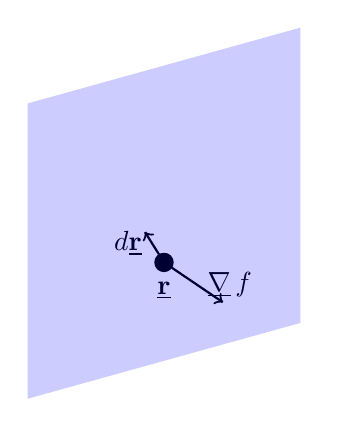
\begin{tikzpicture}[scale=1.25]
   \node[circle,draw,fill=black,label=below:$\vec r$,scale=0.7] (b1) at (1,1,1){};
   \draw[thick,->] (1, 1.5, 1.5) -- node[left]{$d\vec r$} (b1) -- (1, 1.5, 1.5);
    \draw[thick,->] (1.5, 0.5, 0.75) -- node[right]{$\grad$} (b1) -- (1.5, 0.5, 0.75);
   \fill[blue,opacity=0.2] (2,0,0) -- (0,0,2) -- (0,3,2) --  (2,3,0) -- node[midway,right]{} cycle;
  \end{tikzpicture}
\end{figure}

Suppose that $d\vec r$ lies in the level surface $f = C$, then $\displaystyle{d\vec f = \grad\cdot d\vec r = 0}$ so $\grad$ and $d\vec r$ are perpendicular. To show that $\grad$ has the required magnitude, let $d\vec r = \vecn ds$, where $\vecn$ is normal to the surface and $s$ is a distance measured along the normal.
\begin{align*}
  df &= \grad\cdot d\vec r\\
  &= \grad\cdot\vecn ds \\
  &= |\grad|ds
\end{align*}
So we know that $\displaystyle{\grad\parallel ds \implies \frac{df}{ds} = |\grad|}$.

\begin{example}{
   Let $f(x, y, z) = \sqrt{x^2 + y^2 + z^2}$, the euclidean norm.
}\end{example}\begin{solution}{
  Then we know that $\displaystyle{\grad = (\frac{x}{r}, \frac{y}{r} + \frac{z}{r}) = \frac{\vec r}{r}}$, where $r = \sqrt{x^2 + y^2 + z^2}$ and $\vec r = {x} \veci + {y} \vecj + {z} \veck$
}\end{solution}\vspace{10pt}

\section{Directional Derivative}

\begin{figure}[H]
  \centering
  \tdplotsetmaincoords{70}{30}
  \begin{tikzpicture}[tdplot_main_coords]
  \coordinate (O) at (0,0,0);
  \draw[->] (O) --++ (3,0,0) node[below] {$x$};
  \draw[->] (O) --++ (0,3,0) node[below] {$y$};
  \draw[->] (O) --++ (0,0,3) node[right] {$z$};

  \draw[thick,red] (0,0,1) -- (2,1,2) node[right] {$L$};
  \draw[thick,blue, ->] (0,0,0) -- node[right] {$\vec x + t\vec v$} ++ (1.5,0.75,1.75);
  \draw[thick,blue, ->] (0,0,0) -- node[left] {$\vec x$} ++ (0.2,0.1,1.1);
  \draw[very thick,blue] (0.2,0.1,1.1) -- node[above] {$t\vec v$} (1.5,0.75,1.75);
  \end{tikzpicture}
\end{figure}
Suppose $f: \R^3 \to \R$, let $\vec v, \vec x\sub \R^3$ be fixed vectors. Consider the function from $\R\to\R$ defined as:
\begin{equation*}
  t \mapsto f(\vec x + t\vec v)\tag{$\dagger$}
\end{equation*}
The set of points of the form $\vec x + t\vec v$, $t\in \R$ is the line $L$ through which the point $\vec x$ is parallel to $\vec v$. ($\dagger$) is a function, $f$, restricted to $L$.
 \noindent\begin{definition}{Directional Derivative}{}
  If $f: \R^3 \to \R$, the directional derivative of $f$ at $\vec x$ along a vector $\vec v$ is given by:
  $$ \frac{d}{dt}\Bigr|_{t=0}f(\vec x + t\vec v) $$ if it exists.
 \end{definition}\vspace{10pt}
\noindent Note that we usually choose $\vec v$ to be of length unity.

\noindent\begin{theorem}{}{}
  If $f: \R^3 \to \R$ and differentiable, then all directional derivatives exist. The directional derivative at $\vec x$ in direction $\vec v$ is given by:
  $$ \frac{d}{dt}\Bigr|_{t=0}f(\vec x + t\vec v) = \grad(\vec x)\cdot \vec v $$
\end{theorem}\vspace{10pt}
\begin{proof}
  Let $\vec c(t) = \vec x + t\vec v$, $f(\vec x + t\vec v) = f(\vec c(t))$ and
  \begin{align*}
    \frac{d}{dt}\Bigr|_{t=0} f(\vec c (t)) &= \grad(\vec c(t))\cdot \vec c'(t) \\
    &= \grad{\vec c(0)}\cdot \vec c'(0)\\
    &= \grad(\vec x)\cdot\vec v\\
  \end{align*}
\end{proof}

\noindent\begin{theorem}{}{}
   Assume that $\displaystyle{\grad \neq 0}$. Then $\grad(x)$ points in the direction along which $f$ is increasing fastest
\end{theorem}\vspace{10pt}
\begin{proof}
  If $\vecn$ is a unit vector, the rate of change of $f$ in the direction $\vecn$ is given by:
  $$ \grad \cdot \vecn = |\grad||\vecn|\cos{\vartheta} = |\grad|\cos{\vartheta} $$
  where $\vartheta$ is the angle between $\vecn$ and $\grad$. This maximum is when $\th = 0$, so $\vecn$ and $\grad$ are parallel. If we wish to move in the direction in which $f$ decreases the fastest, we should proceed in the direction, $-\grad$.
\end{proof}

\begin{example}{
   Find the unique normal to $\displaystyle{x^2 + y^2 - z = 0}$ at $(1, 1, 2)$
}\end{example}\begin{solution}{
  We say that $f(x, y, z) = x^2 + y^2 - z = 0$, and that $\grad$ is normal as $f$ is a level surface. So:
  $$ \grad = 2x\veci + 2y\vecj - \veck$$
  and we can work out $\vecn$ as:
  $$ \vecn = \frac{(2x, 2y, -1)}{\sqrt{1 + 4(x^2 + y^2)}}\Bigr|_{(1, 1, 2)} $$
  and so $\vecn = \frac{1}{3}(2, 2, -1)$
}\end{solution}\vspace{10pt}

\subsection{Properties of Gradient}
For any scalar functions of $f(x, y, z)$ and $g(x, y, z)$ and any $c\in\R$, we have:
\begin{align*}
  \nab{(f + g)} &= \grad + \nab g\\
  \nab{(cf)} &= c\grad \\
  \nab{(fg)} &= f\nab{g} + g\grad\\
  \nab{(f\circ g)} &= f'(g(x))\nab{g}\\
\end{align*}

\section{Parameterised Curves}
We consider smooth curves in $\R^3$ specified in terms of rectangular cartesian coordinates $(x, y, z)$. Such curves are generated by three smooth functions of a single parameter, $t$.

\begin{example}
   A good example is a circular helix, $r(t) = x(t)\veci + y(t)\vecj + z(t)\veck$, where: $x(t) = a\cos t$, $y(t) = b\sin{t}$ and $z(t) = ct$
\end{example}\vspace{10pt}
\begin{figure}[H]
  \centering
  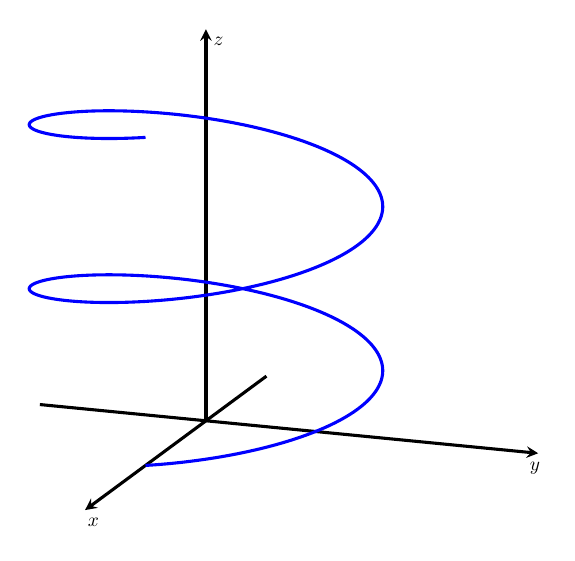
\begin{tikzpicture}[scale=0.7]
  \begin{axis}[
   view={-20}{-20},
   axis line style = ultra thick,
   axis lines=middle,
   zmax=60,
    xmax=2,
     ymax=2,
   height=12cm,
   xtick=\empty,
   ytick=\empty,
   ztick=\empty,
   clip=false,
   x label style={at={(axis cs:2,0.051)},anchor=north},
     xlabel={$y$},
   y label style={at={(axis cs:0.05,2)},anchor=north},
     ylabel={$x$},
   z label style={at={(axis cs:0.075,0,60)},anchor=north},
     zlabel={$z$},
  ]
  \addplot3+[domain=0:4*pi,samples=500,samples y=0,blue,no marks,ultra thick]
  ({sin(deg(x))},
  {cos(deg(x))},
  {4*x});
  %\draw (A)--(B);
  \end{axis}
  \end{tikzpicture}
\end{figure}

We can calculate the length of a path using an integral. Take a function that parameterised with three variables, $x(t), y(t), z(t)$ and between two points, $t_0\le t\le t_1$, we can find the length, L:
$$ L(\vec r) = \int_{t_0}^{t_1}{\sqrt{\dot x^2(t) + \dot y^2(t) + \dot z^2(t)}} $$
We could also parameterise a curve using an arc length parameter, $s$, where differential of arc-length satisfy the equation:
\begin{align*}
  ds^2 &= dr \cdot dr \\
  &= dx^2 + dy^2 + dz^2
\end{align*}
We call $ds$ the line element of the curve. We can also write this with respect to $t$:
$$ \dot s^2 = \dot x^2 + \dot y^2 + \dot z^2 = \dot r \cdot \dot r$$
Now we have a curve in a space $\vec r(t)$. Then we can find a tangent, $\dot{\vec r} = (\dot x, \dot y, \dot z)$, which then we know that $\displaystyle{|\dot{ \vec r}| = \dot s}$ and $\displaystyle{\hat{\vec t} = \frac{\dot{\vec r}}{|\dot{\vec r}|}}$. We have now swapped the parameter from $t$ to $s$.
$$ \hat{\vec t} = {\frac{dx}{ds}} \veci + {\frac{dy}{ds}} \vecj + {\frac{dy}{ds}} \veck $$
As we then know that $\hat{\vec t}$ is a unit vector, $\hat{\vec t}\cdot\hat{\vec t} = 1$, now differentiate and $\displaystyle{\hat{\vec t} \cdot \frac{d\hat{\vec t}}{ds} = 0}$, hence $\displaystyle{\frac{d\hat{\vec t}}{ds}} \perp \hat{\vec t}$. The $\frac{d\hat{\vec t}}{ds}$ is in the direction of the principle normal, $\vec n$, of the curve. So $\frac{d\hat{\vec t}}{ds} = \kappa(s)\vecn$\\

The plane spanned by $\hat{\vec t}(s)$ and $\vecn(s)$ is the osculating plane.\\

So if we have a curve $\vec r(t)\in \R^3$, then $\displaystyle{\fd{\vec r}{t}}$, so we can now say that $\displaystyle{\frac{\dot{\vec r(t)}}{|\dot{\vec r (t)}|} = \fd{\vec r}{s} = \uvec{t}}$. Now we can take derivatives and hence:
$$ \fd{\uvec t}{s} = \kappa \vecn $$

Moving forward now, we can take $\displaystyle{\uvec t = \vec r'(s)}$ and then differentiating: $\displaystyle{\uvec t = \vec r''(s)}$, which then implies:
$$ \kappa = |\vec r''(s)| $$
and then we know that $\displaystyle{\dot{\vec r}(t) = \vec r'(s)\dot{s}}$
 and then $\displaystyle{\ddot{\vec r(t)} = r''\dot{s}^2 + \frac{\ddot{s}}{\dot{s}}\dot{\vec r}}$ and hence we can say that: $\displaystyle{\vec r''(s) = \frac{1}{\dot{s}^2}\ddot{\vec r} - \frac{\ddot{s}}{\dot{s}^3}\dot{\vec r}}$. So now,
 $$ \kappa^2(s) = \frac{1}{(\dot{\vec r}\cdot\dot{\vec r})^3}\big((\ddot{\vec r}\cdot\ddot{\vec r})(\dot{\vec r}\cdot\dot{\vec r}) - (\dot{\vec r}\cdot\ddot{\vec r})^2) $$

 Given a unit tangent vector, $\uvec t$ and a unit normal vector, $\vecn$ at a point on a curve in $\R^3$, we can define a third unit vector $\uvec{b}$ which is the unit binormal vector.
 $$ \uvec b = \uvec t \times \vecn$$
 They form a right handed system of unit vectors, this forms the moving trihedron as $s$ varies.
 $$ \uvec b = \uvec t \times \uvec n,\quad \uvec n = \uvec b \times \uvec t,\quad \uvec t = \uvec n \times \uvec b $$

\subsection{Deriving Frenet-Serret Equations}


 We can now differentiate the other two equations, and get; $\displaystyle{\fd{\uvec b}{s}\perp \uvec b}$ and
\begin{align*}
  \fd{\uvec b}{s} &= \fd{\uvec t}{s} \times \uvec n + \uvec t \times \fd{\uvec n}{s} \\
  &= \k\uvec n \times \uvec n + \uvec t\times \fd{\uvec n}{s} \\
  &= \uvec t \times \fd{\uvec n}{s}\\
\end{align*}
which also tells us that:
$$ \fd{\uvec b}{s} \perp \uvec t, \fd{\uvec n}{s} $$
and hence $\displaystyle{\fd{\uvec n}{s} \parallel \vecn}$ and so,
$$ \fd{\uvec b}{s} = -\tau \uvec n $$
we call, $\tau$ the torsion of the curve.

\begin{example}{
 We shall take the helix again,
 \begin{align*}
   d\vec r &= -a\sin t dt\veci + a\cos t dt\vecj + c dt\veck\\
   ds ^2 &= (a^2 (\sin^2 t + \cos^2 t) + c^2) dt^2 \\
   ds &= (a^2 + c^2)^{\frac{1}{2}}dt  \\
   &\implies t = (a^2 + c^2)^{-\frac{1}{2}}s\\
 \end{align*}
  Now we can find the tangent to any point.
  $$ \vec r'(s) = \frac{1}{\sqrt{a^2 + c^2}}\left( -a\sin{\frac{s}{\sqrt{a^2 + c^2}}}\veci + a\cos{\frac{s}{\sqrt{a^2 + c^2}}}\vecj + c\veck\right) $$
  and now for $\uvec t'(s)$
  $$ \uvec t' = \vec r''(s) = \frac{a}{{a^2 + c^2}}\left( -\cos{\frac{s}{\sqrt{a^2 + c^2}}}\veci - \sin{\frac{s}{\sqrt{a^2 + c^2}}}\vecj \right) $$
  comapring both sides, we can say that: $\displaystyle{\k(s) = \frac{a}{a^2 + c^2}}$. Finally, we find $\uvec b(s)$ as:
  $$ \uvec b = \uvec t\times\uvec n = \frac{1}{\sqrt{a^2 + c^2}}\left( -c\sin{\frac{s}{\sqrt{a^2 + c^2}}}\veci - c\cos{\frac{s}{\sqrt{a^2 + c^2}}}\vecj + a\veck\right) $$
  and to find torsion:
  $$ \uvec b' = \frac{c}{{a^2 + c^2}}\left( \cos{\frac{s}{\sqrt{a^2 + c^2}}}\veci + \sin{\frac{s}{\sqrt{a^2 + c^2}}}\vecj + a\veck\right) $$
  and so torsion:
  $$ \tau(s) = \frac{c}{a^2 + c^2} $$
}\end{example}
Now for $\uvec n$, we can differentiate once and get:
\begin{align*}
  \fd{\uvec n}{s} &= \fd{\uvec b}{s}\times\uvec t + \uvec b\times \fd{\uvec t}{s} \\
  &= -\tau(s)\uvec n\times \uvec t + \uvec b\times\k\uvec n \\
  &= \tau(s)\uvec b - \k(s)\uvec t
\end{align*}

\noindent\begin{definition}{Frenet-Serret Equations in $\R^3$}{}
  \begin{equation*}
      \fd{\uvec t(s)}{s} = \k(s)\uvec n(s)\\
    \end{equation*}
    \begin{equation*}
      \fd{\uvec b(s)}{s} = -\tau(s)\uvec n(s)\\
      \end{equation*}
      \begin{equation*}
      \fd{\uvec n(s)}{s} = \tau(s)\uvec b - \k(s)\uvec t\\
  \end{equation*}
\end{definition}\vspace{10pt}

If you are given $\uvec t$, $\uvec n$, $\k$ and $\tau$, you can use the Frenet Serret equations to determine $\uvec t$, $\uvec n$ and $\uvec b$ and thus determine the curve in its entirity.

\newpage
\section{Differentiation and Vector Fields}
If $\vec A(t) = {A(t)}_1 \veci + {A(t)}_2 \vecj + {A(t)}_3 \veck$, then:
$$ \fd{\vec A(t)}{t} = {\fd{\vec A(t)}{t}}_1 \veci + {\fd{\vec A(t)}{t}}_2 \vecj + {\fd{\vec A(t)}{t}}_3 \veck $$
and let $\p = \p(x, y, z, t)$, $\vec A(\vec x, t)$, $B(\vec x, t)$, then:
\begin{align}
  \pd{}{t}(\p \vec A) &= \pd{\p}{t}\vec A + \p\pd{\vec A}{t} \tag{$*$}\\
  \pd{}{t}(\vec A + \vec B) &= \pd{\vec A}{t} + \pd{\vec B}{t} \tag{$*^2$}\\
  \pd{}{t}(\vec A \cdot \vec B) &= \pd{\vec A}{t}\cdot\vec B + \vec A \cdot\pd{\vec B}{t} \tag{$*^3$}\\
  \pd{}{t}(\vec A \times \vec B) &= \pd{\vec A}{t}\times\vec B + \vec A\times\pd{\vec B}{t} \tag{$*^4$}
\end{align}
Now for the second derivatives
\begin{align*}
  \pd{^2 \vec A}{x\pa y} &= \pd{^2 \vec A}{y\pa x} \\
  &= \pd{}{x}\left(\pd{\vec A}{y} \right)\\
  &= \pd{^2 \vec A_1}{x\pa y}\veci + \pd{^2 \vec A_2}{x\pa y}\vecj + \pd{^2 \vec A_3}{x\pa y}\veck \\
\end{align*}

\subsection{Divergence of a vector field}
The divergence of a vector field $\displaystyle{u(\vec x, t)}$ is a scalar field. It's value at a point $P$ is defined:
$$ \div u = \lim_{\de \vec V \to 0}{\oiint{\vec u \cdot \vec n}ds}  $$
where $\vec V$ is a small volume enclosing $P$. Physically this is the amount of flux in vector field, $\vec U$ out of $\de \vec V$ divided by the volume.
$$ \div \vec u = \pd{\vec u_1}{x} + \pd{\vec u_2}{y} + \pd{\vec u_3}{z} $$
Assume $P(x, y, z)$ is enclosed by a cube of side length, $\de x, \de y, \de z$. Assume $P$ is at the centre of the cube. Then:
\begin{align*}
  \oiint_S \vec u \cdot\vec n ds &= \iint_{S_1} \vec u \cdot\vec n ds + \iiint_{S_2} \vec u \cdot\vec n ds + \iint_{S_3} \vec u \cdot\vec n ds\\
  &\quad+ \iint_{S_4} \vec u \cdot\vec n ds +\iint_{S_5} \vec u \cdot\vec n ds + \iint_{S_6} \vec u \cdot\vec n ds\\
  &= u_1 (x +\frac{\de x}{2}, y, z)\de y \de z - u_1 (x -\frac{\de x}{2}, y, z)\de y \de z \\
  &\quad+ u_2 (x, y +\frac{\de y}{2}, z)\de x \de z - u_2 (x , y-\frac{\de y}{2}, z)\de x \de z \\
  &\quad+ u_3 (x, y, z+\frac{\de z}{2})\de x \de y - u_3 (x , y, z-\frac{\de z}{2})\de x \de y \\
  &= \pd{u_1}{x}\de \vec V + \pd{u_2}{y}\de \vec V + \pd{u_3}{z}\de \vec V\\
\end{align*}
So we can conclude that:
$$ \lim_{\de \vec V \to 0}{\oiint{\vec u \cdot \vec n}ds} = \pd{u_1}{x} + \pd{u_2}{y} + \pd{u_3}{z} = \div\vec u$$

\noindent\fbox{\parbox{0.475\textwidth}{\begin{example}{
 Compute divergence of $F = x^2y\veci + z\vecj + xyz\veck$
}\end{example}\begin{solution}{
\begin{align*}
  \div F &= \pd{}{x}(x^2y) + \pd{}{y}(z) + \pd{}{z}(xyz)\\
  &= 3xy
\end{align*}
}\end{solution}}}\vspace{10pt}

\section{Curl of a Vector Field}
The curl of a vector field $\vec u (\vec x, t)$ is a vector field. The component in the direction of the $\vecn$,
$$ \vecn \cdot \curl \vec u = \lim_{\de S\to 0}{\frac{1}{\de S}\oint_{\de C}{\vec u \cdot d\vec r}} $$
$\curl \vec u$ is related to the rotatio or tisting of the vector field.
$$ \curl \vec u = \left |\begin{matrix}
  \veci & \vecj & \veck \\
  \pd{}{x} & \pd{}{y} & \pd{}{z} \\
  u_1 & u_2 & u_3 \\
\end{matrix}\right | = $$
To prove this:
\begin{align*}
  \vecn \cdot \curl \vec u &= \lim_{\de S\to 0}{\frac{1}{\de S}\oint_{\de C}{\vec u \cdot d\vec r}}\\
  &= \oint_{C_1}{\vec u \cdot d\vec r} + \oint_{C_2}{\vec u \cdot d\vec r} \\
  &\quad+ \oint_{C_3}{\vec u \cdot d\vec r} + \oint_{C_4}{\vec u \cdot d\vec r}\\
  &\approx u_1(x, y - \frac{\de y}{2}, z)\de x + - u_1(x, y + \frac{\de y}{2}, z)\de x\\
  &\quad+ u_2(x + \frac{\de x}{2}, y, z)\de y - u_2(x - \frac{\de x}{2}, y, z)\de y \\
  &= -\pd{u_1}{y}\de y\de x + \pd{u_2}{x}\de x\de y \\
  &= \pd{u_2}{x} - \pd{u_1}{y}
\end{align*}
The other components of $\curl \vec u$ can be found with similar arguments. 
















\end{document}
